\documentclass[english]{article}
\usepackage[T1]{fontenc}
\usepackage[latin9]{inputenc}
\usepackage{babel}
\usepackage{graphicx}
\usepackage{subfigure}
\usepackage{float}
\setlength{\parindent}{0pt}
\usepackage{amsmath}


\begin{document}

\title{Lab 4: Compact Vision System\\ -------------------------------- \\ \Large Sensors and Digitization}
\author{ \ Armine Vardazaryan, Songyou Peng \\ arminevardazaryan@gmail.com, psy920710@gmail.com}
\date{9rd December 2015}

\maketitle

\section{Introduction}

\section{Edge Detection}
\section{Caps Detection}
In this part, we try to program to detect perfume caps.
If the system can tell whether the perfume caps are there or not, then we can say it is a successful system for cap detection.\\
\\
First, we set "Measure" to "Multi pattern position".
Second, we manually give a search window in the image so that the detection system can only search the object in the search window (blue triangle in Figure \ref{fig:window}).
Then we set pattern window for perfume cap, which is the white triangle shown in the Figure \ref{fig:window}.

\begin{figure}[H]
	\centering
	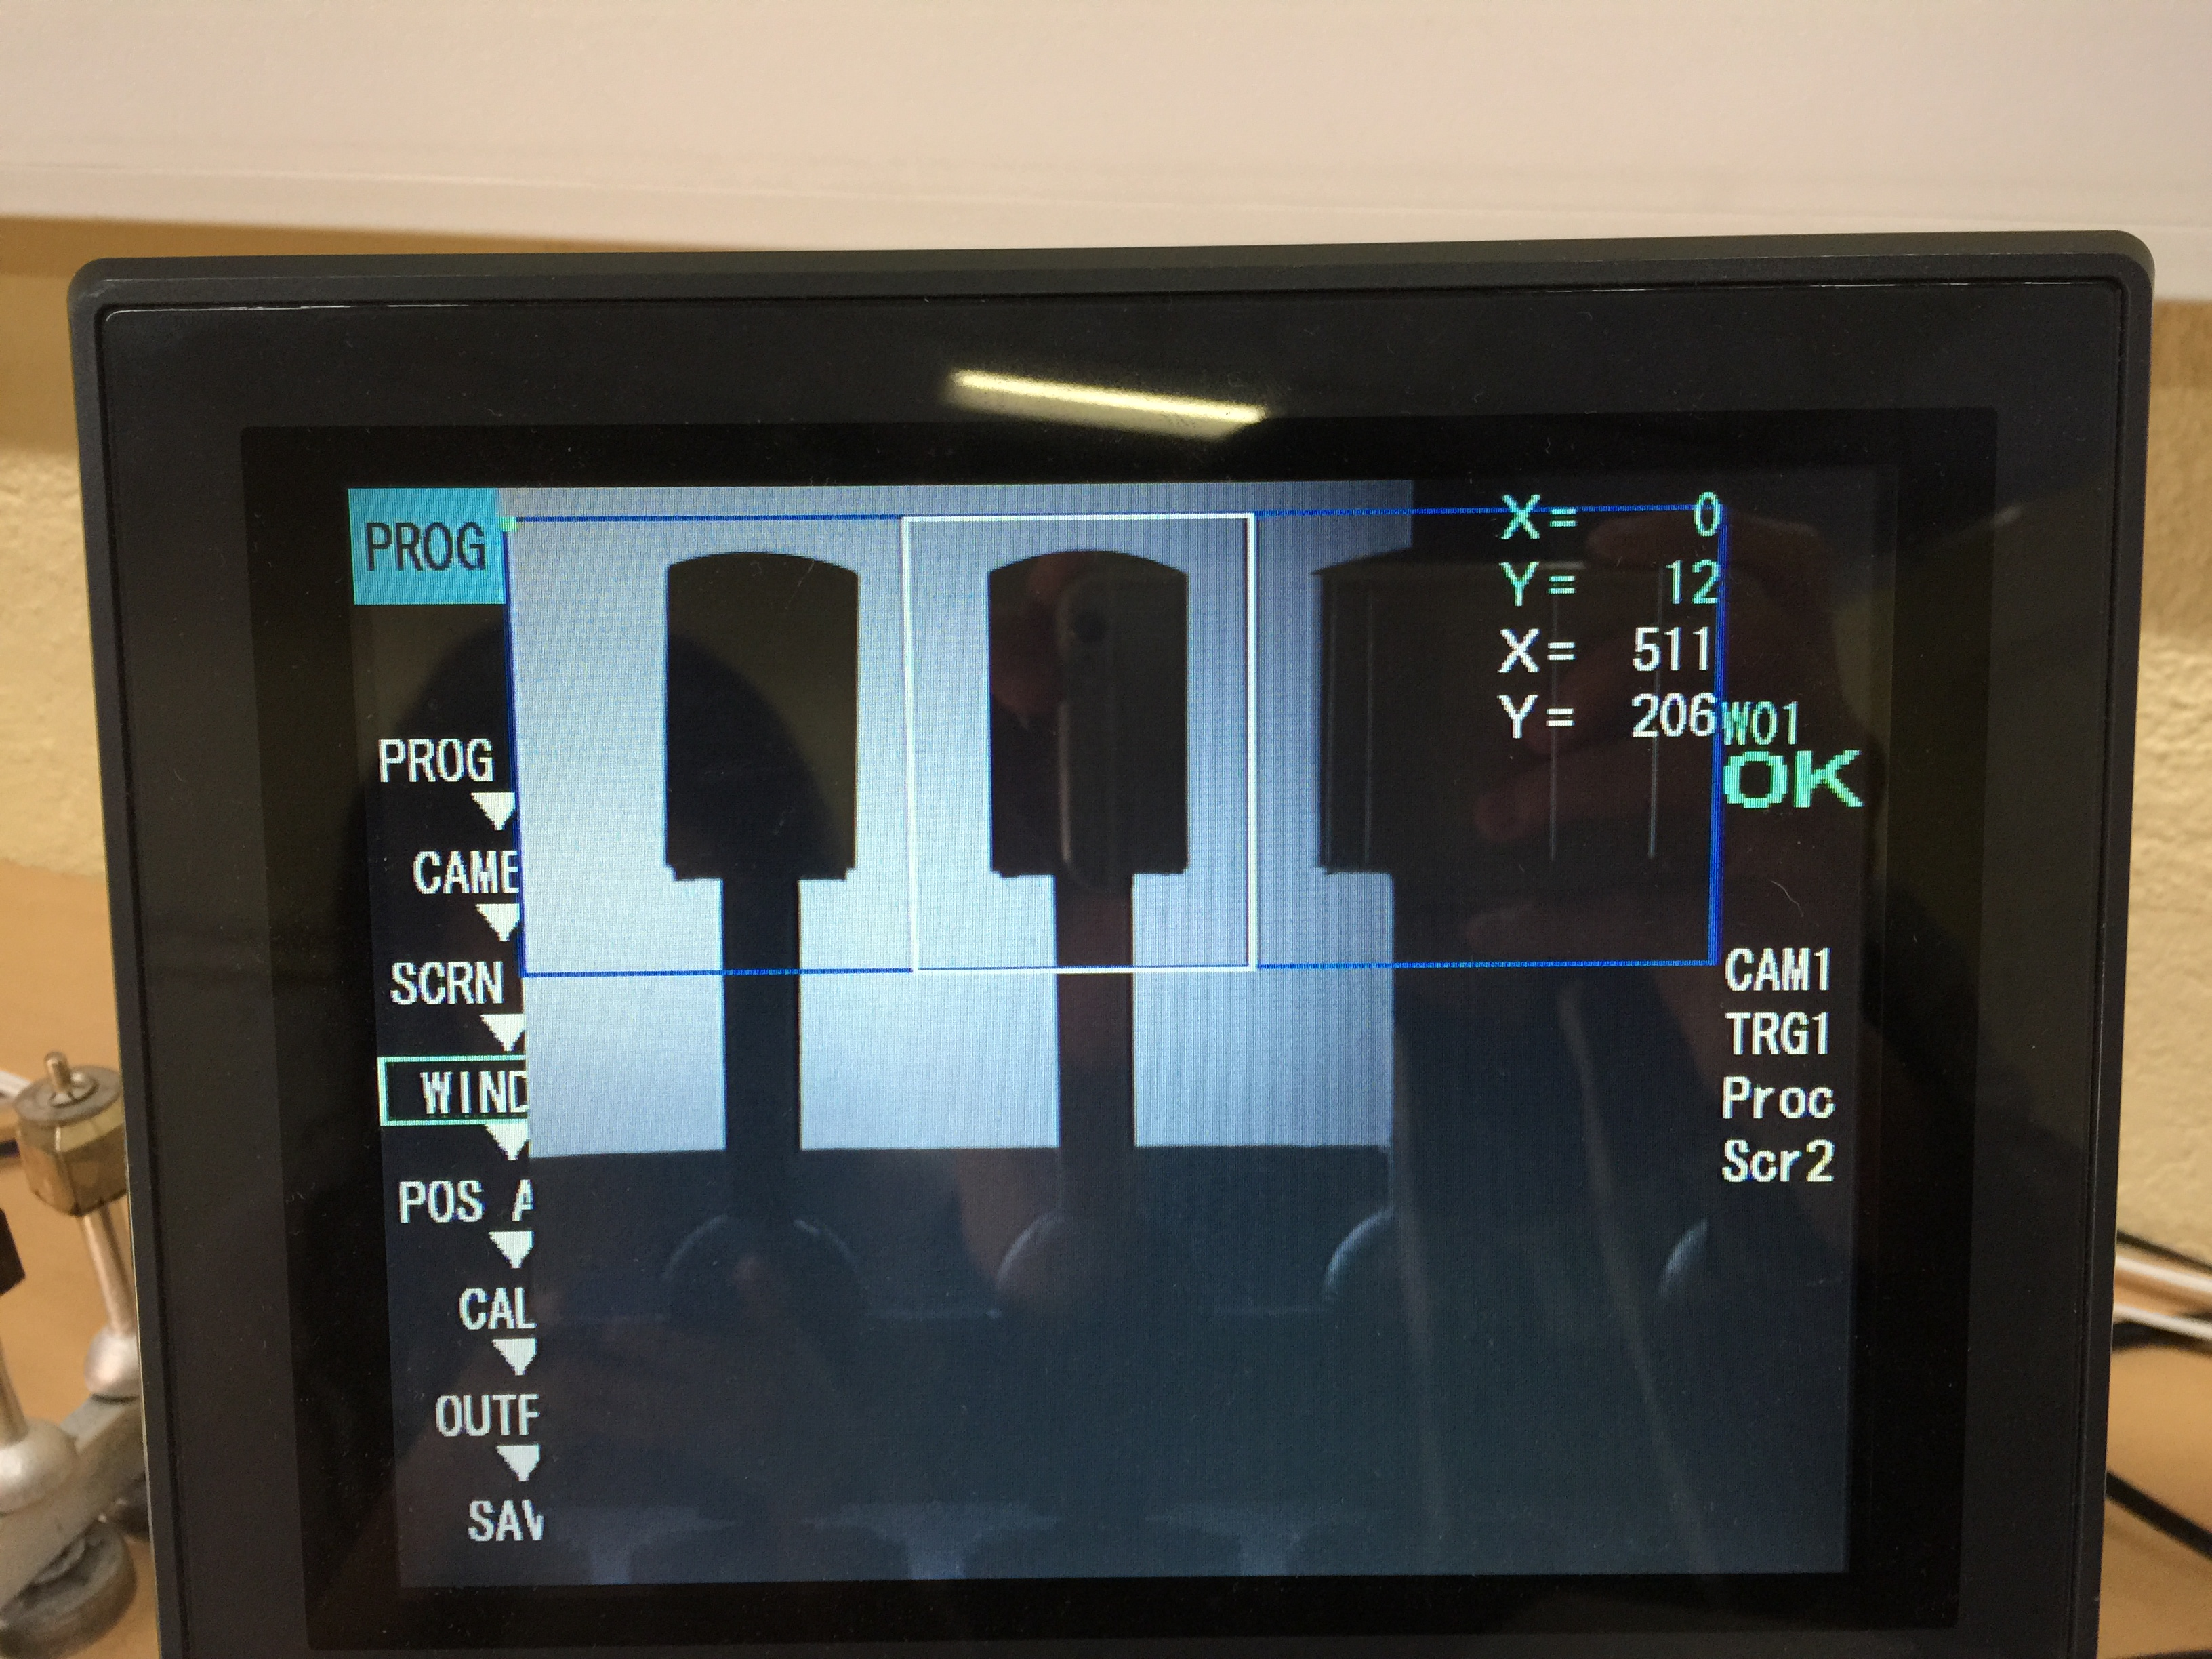
\includegraphics[width=0.45\linewidth]{Pictures/IMG_1225.JPG}
	\caption{Search window (blue) and pattern window (white)}
	\label{fig:window}
\end{figure} 

After setting up all the configuration, we start to use external trigger to grab pictures of outcome of detection (Figure \ref{fig:caps}). In the Figure \ref{fig:capsa}, we are able to see our detection system distinguish two caps in the search window, while in the Figure \ref{fig:capsb}, the system also figure out the cap correctly.\\
\\
In order to check the robustness of the system, we rotate the caps to different angle (Figure \ref{fig:capsc}), and the system can still tell the difference. It turns out the system is robust enough.

\begin{figure}[H]
	\centering
	\subfigure[Two caps]{\label{fig:capsa}
	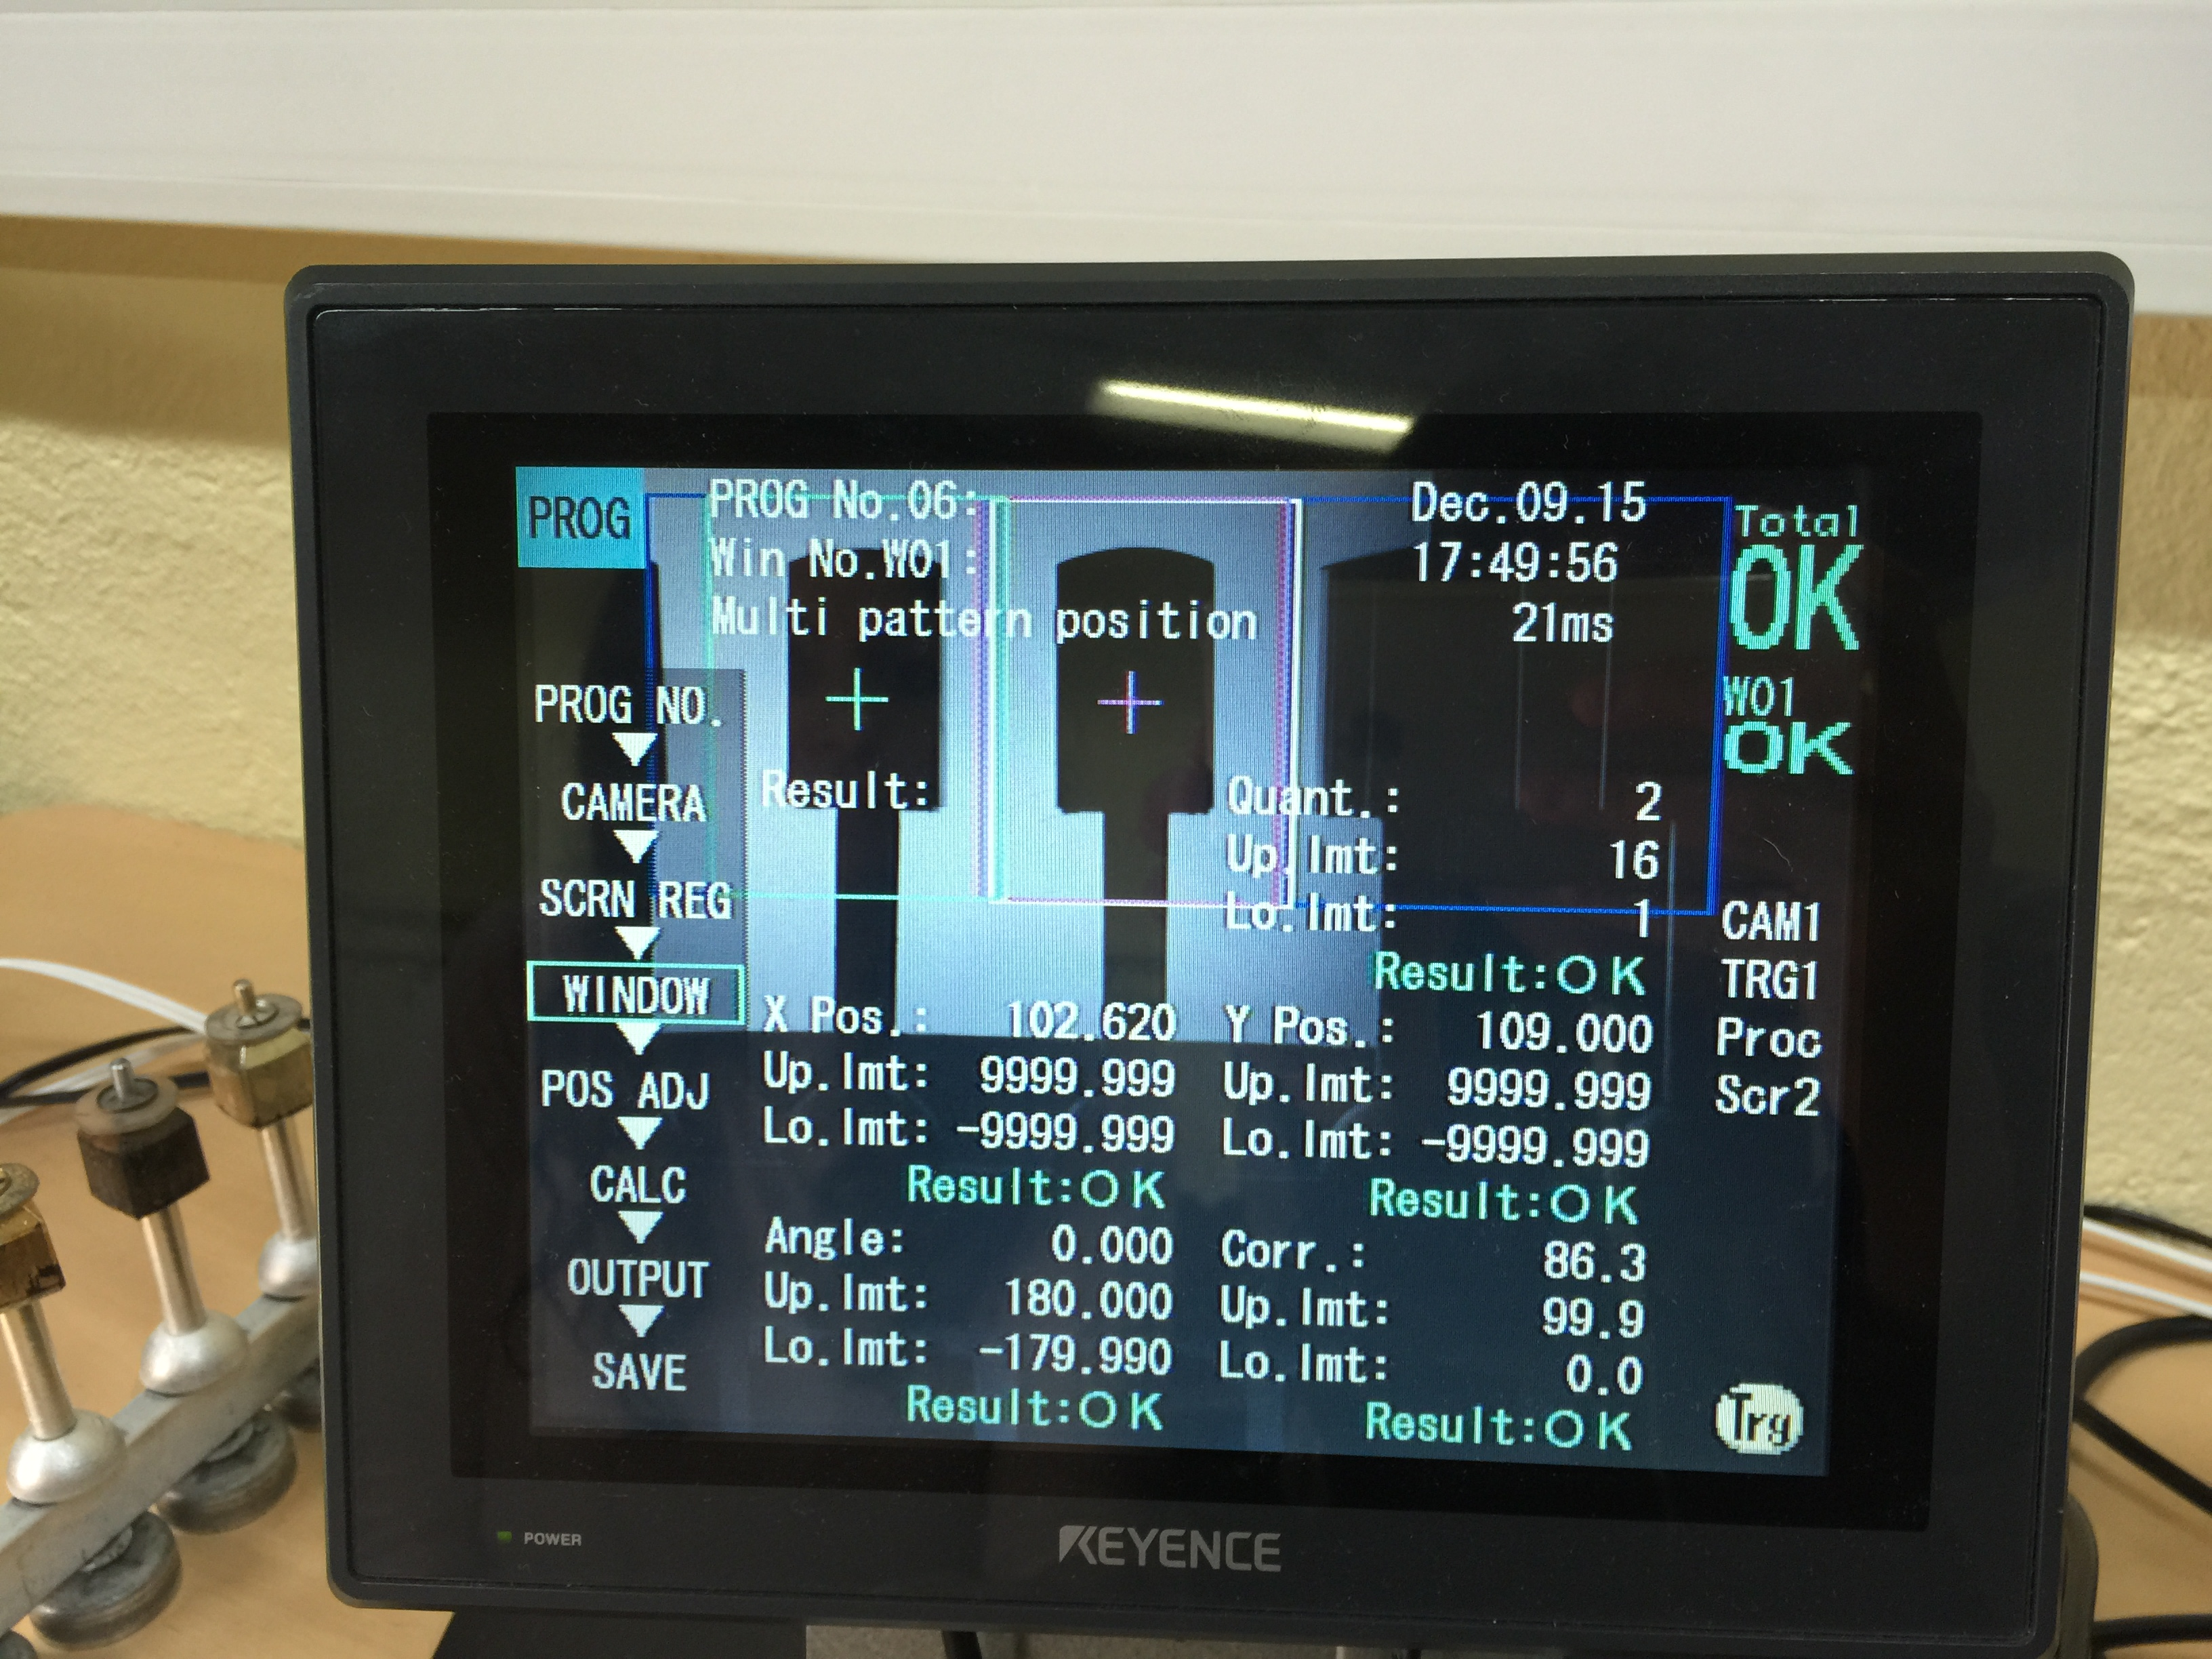
\includegraphics[width=0.45\linewidth]{Pictures/IMG_1226.JPG}
	}
	\subfigure[One caps]{\label{fig:capsb}
	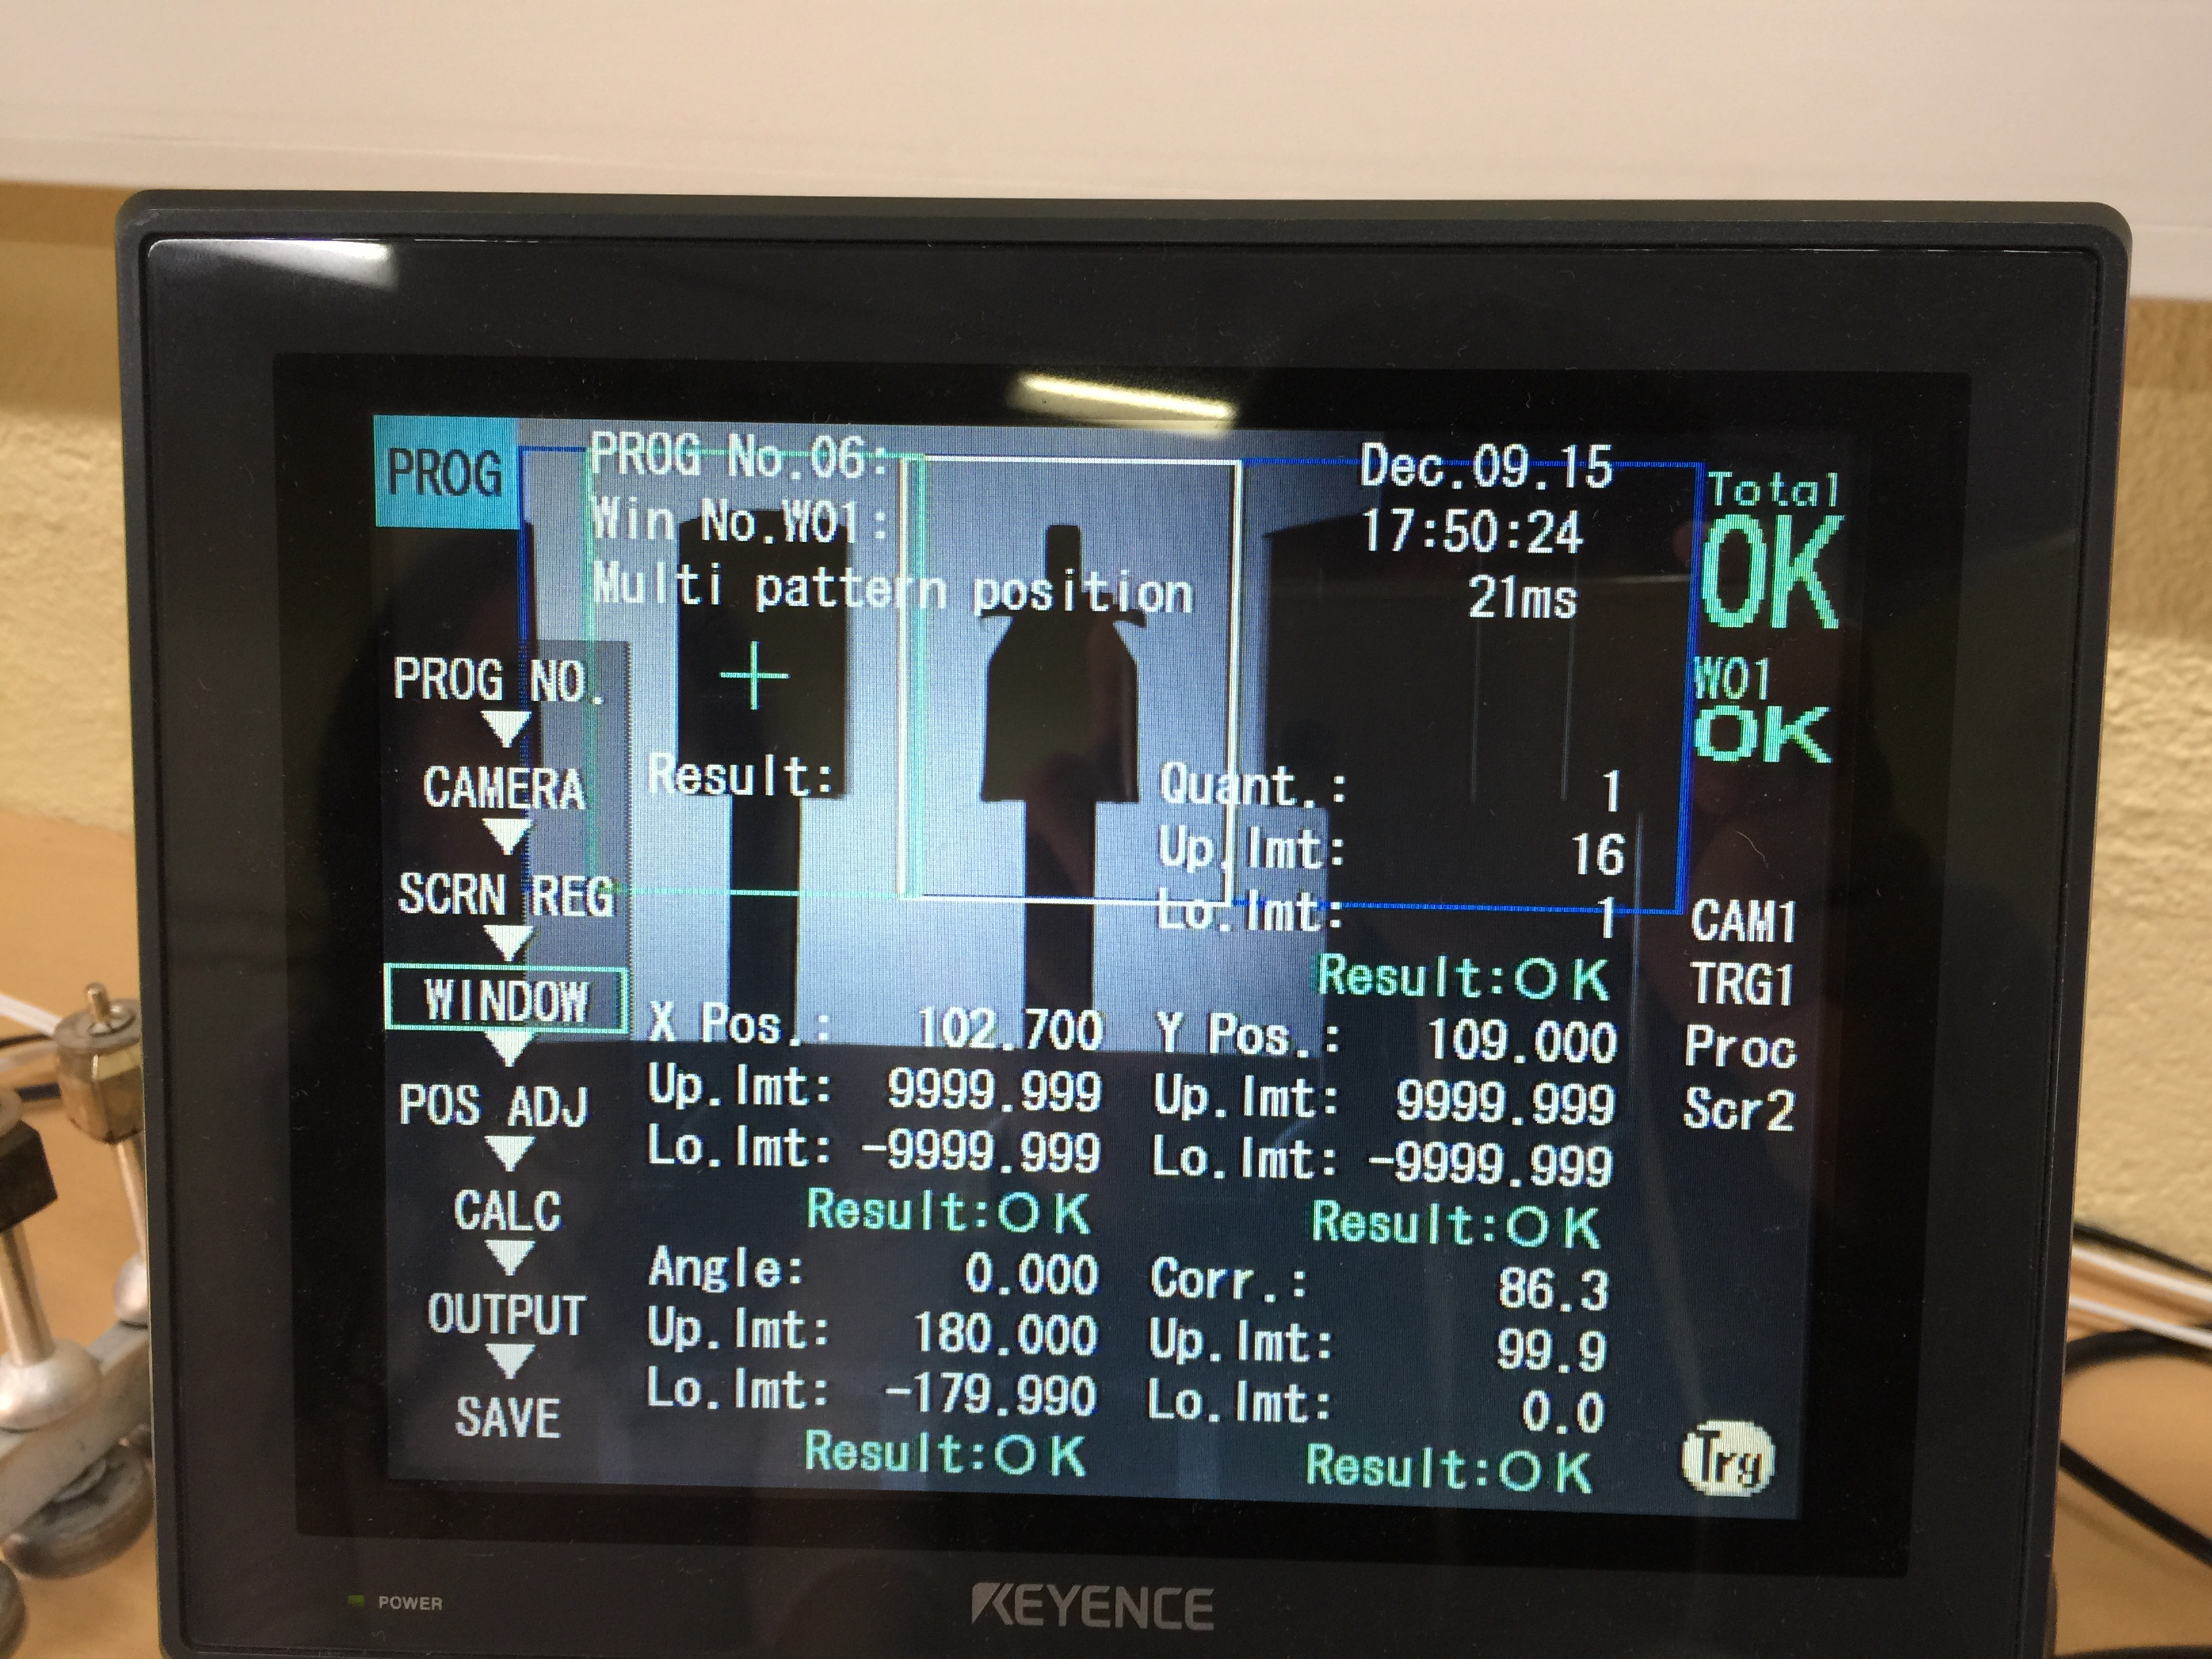
\includegraphics[width=0.45\linewidth]{Pictures/IMG_1227.JPG}
	}
	\subfigure[Rotate caps]{\label{fig:capsc}
	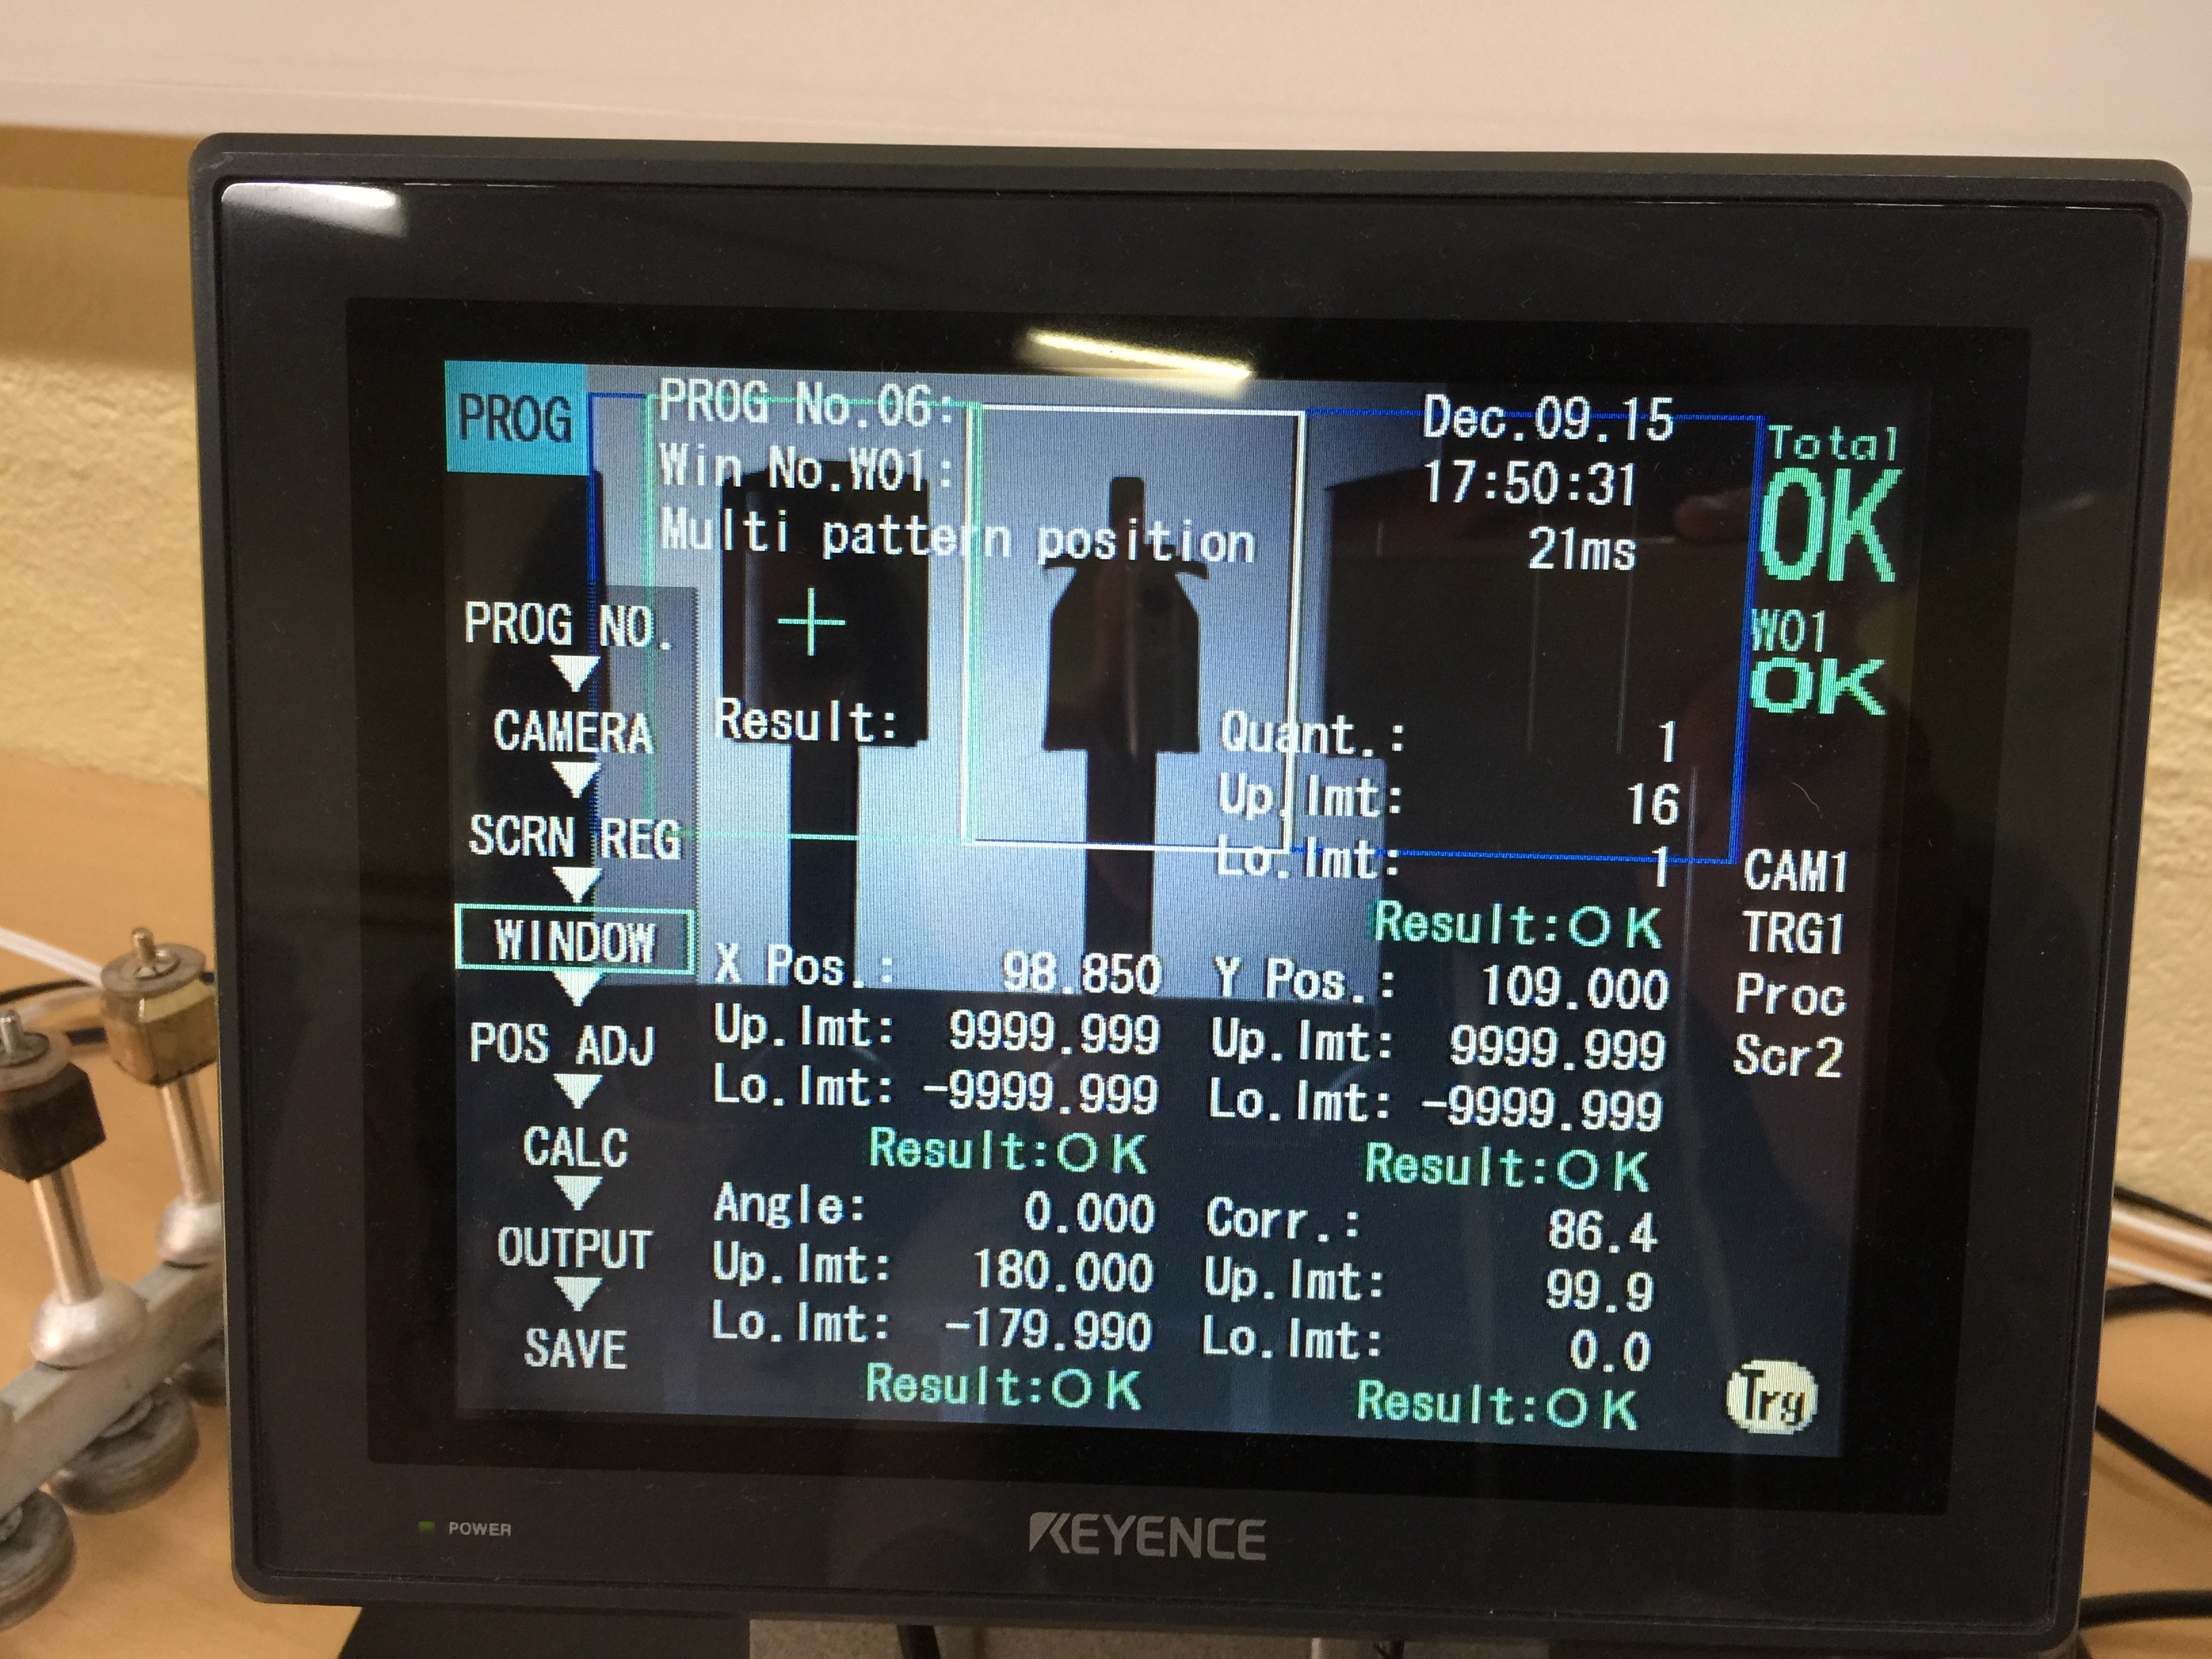
\includegraphics[width=0.45\linewidth]{Pictures/IMG_1228.JPG}
	}
	\caption{Caps detection}
	\label{fig:caps}
\end{figure}

\section{Conclusion}
In this lab, we learn and program a Compact Vision System from KEYENCE. First we program to find the edge of objects and count the number. Second, we select proper tools and  create another detection system to detect whether the perfume caps is in the object.
\section{References}

\end{document}